%%%%%%%%%%%%%%%%%%%%%%%%%%%%%%%%%%%%%%%%%
% Beamer Presentation
% LaTeX Template
% Version 1.0 (10/11/12)
%
% This template has been downloaded from:
% http://www.LaTeXTemplates.com
%
% License:
% CC BY-NC-SA 3.0 (http://creativecommons.org/licenses/by-nc-sa/3.0/)
%
%%%%%%%%%%%%%%%%%%%%%%%%%%%%%%%%%%%%%%%%%

%----------------------------------------------------------------------------------------
%	PACKAGES AND THEMES
%----------------------------------------------------------------------------------------


\documentclass{beamer}

\mode<presentation> {
\usetheme{Madrid}

\setbeamertemplate{footline}[page number] % To replace the footer line in all slides with a simple slide count uncomment this line
\setbeamertemplate{navigation symbols}{} % To remove the navigation symbols from the bottom of all slides uncomment this line
}

\usepackage{graphicx} 
\usepackage{booktabs}
\usepackage[T1]{fontenc}
\usepackage{amsmath}
\usepackage{mathtools}
\usepackage{amssymb}
\usepackage{graphicx}
\usepackage{graphics}
\usepackage{algorithmic}
\usepackage{algorithm}
\usepackage{listings}
\graphicspath{ {pictures/} } 

\lstset{ 
	basicstyle=\footnotesize, 
	tabsize=2 
} 
%----------------------------------------------------------------------------------------
%	TITLE PAGE
%----------------------------------------------------------------------------------------

%\title[Short title]{Full Title of the Talk} % The short title appears at the bottom of every slide, the full title is only on the title page
\title[]{Cayley graphs of given degree and diameter on linear groups} % The short title appears at the bottom of every slide, the full title is only on the title page

\author{Mat\'u\v{s} Behun} % Your name
\institute[UCLA] % Your institution as it will appear on the bottom of every slide, may be shorthand to save space
{
Slovak University of Technology in Bratislava \\ % Your institution for the title page
\medskip
%\textit{john@smith.com} % Your email address
}
\date{\today} % Date, can be changed to a custom date

\begin{document}

\begin{frame}
\titlepage 
\end{frame}

\begin{frame}
\frametitle{Overview}
\tableofcontents
\end{frame}

%------------------------------------------------
% DEGREE DIAMETER
\section{Degree/diameter} 
%------------------------------------------------

\begin{frame}
	\frametitle{Motivation}
\begin{itemize}
    \item In it's simplest form, networks can be modeled by graphs with nodes as vertices and links between them as edges.
	\item In design of graphs we can take many restrictions into acount such degree, grith, diameter.
	\item Two important problems concerning degree and diameter and degree and grith of graph
\end{itemize}
\end{frame}
%------------------------------------------------
\begin{frame}
\frametitle{The degree/diameter problem}
	\begin{block}{Degree/diameter problem}
		Find graph with biggest possible number of vertices with given degree and diameter.
	\end{block}
\end{frame}
%------------------------------------------------
\begin{frame}
	\frametitle{Moore bound}
There is theoretical upper bound for largest order of graph with $d$-degree and $k$-diameter.
\begin{equation}\label{eq:Moore}
	\begin{split}
		n_{d,k} \leq M_{d,k}    & = 1 + d + d(d - 1) + \dots + d(d - 1)^{k-1}  \\
								& = 1 + d(1 + (d - 1) + \dots + (d - 1)^{k-1}) \\
                                & = \begin{cases}
                                        1+d\frac{(d-1)^{k}-1}{d-2}, & \text{if}\ d > 2 \\
                                    	2k+1, & \text{if}\ d=2
    								\end{cases}
    \end{split}
\end{equation}
\end{frame}
%------------------------------------------------
\begin{frame}
	\frametitle{Moore bound}
		\begin{figure}[!ht]
    		\centering
    		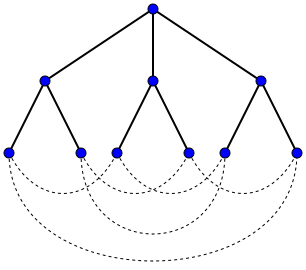
\includegraphics[scale=0.6]{petersen-moore.png}
    		\caption{Peterssen graph is Moore graph with $d=3$ and $k=2$ }
		\end{figure}
\end{frame}
%------------------------------------------------
\begin{frame}
	\frametitle{Moore graphs}
	Graphs with order equal Moore bound are called Moore graphs and are reached only in few cases.	
	\begin{itemize}
		\item If $d = 2$ for any $k \geq 1$
		\item If $k = 1$ for any $d \geq 2$
		\item For $k = 2$ for $d \in \{3, 7 \}$, and possibly $57$
	\end{itemize}
	For other cases we try to construct graphs with order as close to Moore bound as possible.
\end{frame}
%------------------------------------------------
\begin{frame}
	\frametitle{Moore graphs}
	\begin{figure}[!ht]
 		\centering
 		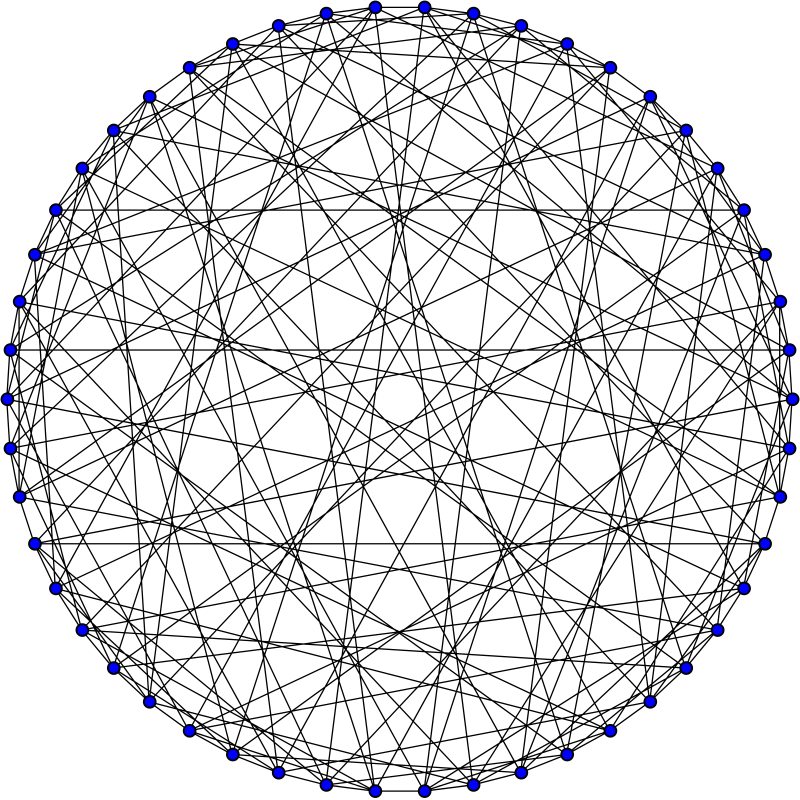
\includegraphics[scale=0.25]{Hoffman-Singleton_graph.png}
		\caption{Hoffman-singleton graph is Moore graph with $d=7$ and $k=2$ }
	\end{figure}
\end{frame}
%------------------------------------------------
% DEGREE DIAMETER
\section{Graph lifting and Cayley graphs} 
%------------------------------------------------
\begin{frame}
	\frametitle{Graph lifting}
	Let $G$ be an undirected graph. We will assign direction to every edge of graph and making them {\em arcs}. {\em Arc} with {\em reversed} direction of $e$ is denoted by $e^{-1}$. 
	\begin{definition}[Graph lifting]
		Let $G$ be a graph as above and let $\Gamma$ be a finite group. The mapping
		\begin{align*}
			\alpha: D(G) \rightarrow \Gamma
		\end{align*}
		will be called a {\em voltage assignment} if $\alpha(e^{-1})$ = $(\alpha(e))^{-1}$, for any arc $e \in D(G)$.
	\end{definition}
\end{frame}
%------------------------------------------------
\begin{frame}
	\frametitle{Graph lifting example}
	Obrazok zdvihu na petersenov graf.
\end{frame}
%------------------------------------------------
\begin{frame}
	\frametitle{Cayley graphs}
	Let $\Gamma$ be a group and let $S\subset \Gamma$ be a symmetric unit-free generating set for $\Gamma$; that is, we require that $S=S^{-1}$ and $1\notin S$. 
	\begin{definition}[Cayley graphs]
		The $\textit{Cayley graph}$ $C(\Gamma,S)$ is the graph with vertex set $\Gamma$ in which vertices $a,b$ are adjacent if $a^{-1}b\in S$. 		
	\end{definition}
\end{frame}
%------------------------------------------------
\begin{frame}
	\frametitle{General linear and Special linear groups}
		\begin{definition}[General linear group] Let $q$ be a power of a prime and let $GF(q)$ be the Galois field of order $q$. The {\em general linear group} $GL(m,q)$ consists of all non-singular $m\times m$ matrices over $GF(q)$ under multiplication of matrices.
		Special linear group is subgroup of $GL(m,q)$ consiting of matrices with determinant equal to 1.
		\end{definition}
		\begin{theorem}[Order of $GL(m,q)$]
			$|GL(m,q)| = (q^m - 1)(q^m - q) \cdots (q^m - q^{n-1})$
		\end{theorem}
		\begin{theorem}[Order of $SL(m,q)$]
			$|SL(m,q)| = |GL(m,q)|/(q-1)$
		\end{theorem}
\end{frame}
%------------------------------------------------
% DEGREE DIAMETER
\section{Computer search of graphs} 
%------------------------------------------------
\begin{frame}
	\frametitle{Computer search of Cayley graphs}
	In order to find graphs with given $d$ and $k$ we generted Cayley graphs from random symmetric unit-free sets $S$ of $SL(2,5)$. 
	\medskip
	With assumptions that: 
	\begin{itemize}
		\item Generating sets yield all elements of $|SL(2,5)| = 120$
		\item Cayley graphs are regular with with $d=|S|$
	\end{itemize}
	we know by Moore bound that size of $S$ must be at least $12$ and all we have to check is diameter of graph. 
\end{frame}
%------------------------------------------------
\begin{frame}
	\frametitle{Computer search of Cayley graphs}
	With one involution in $SL(2,5)$ and with unit-free property of symmetry we have $59$ pairs of elements with its inverses. To check all graphs for $d=12$ we have to generate and check diameter on ${59 \choose 6} = 45057474$ graphs. \\
	In our computation we generated 150000 graphs for all listed degrees. \\
	\begin{tabular}[htbp]{l*{10}{c}r}
		$d$ & $13$ & $14$ & $15$ & $16$ & $17$ & $18$ & $19$ & $20$ & $21$ \\
		\hline
 		Found graphs & $0$  & $0$ & $1$ & $107$ & $345$ & $2451$  & $4120$ & $11669$ & $14926$ \\
	\end{tabular} 
\end{frame}
%------------------------------------------------
\begin{frame}
	\frametitle{Algorithm for generation of cayley graph}
	Algoritmus na generovanie grafu
\end{frame}
%------------------------------------------------
\begin{frame}
	\frametitle{Algorithm for diameter}
	Algoritmus na kontrolu priemeru grafu
\end{frame}
%------------------------------------------------
\begin{frame}
	\frametitle{Output of program}
	\begin{figure}[!ht]
 		\centering
 		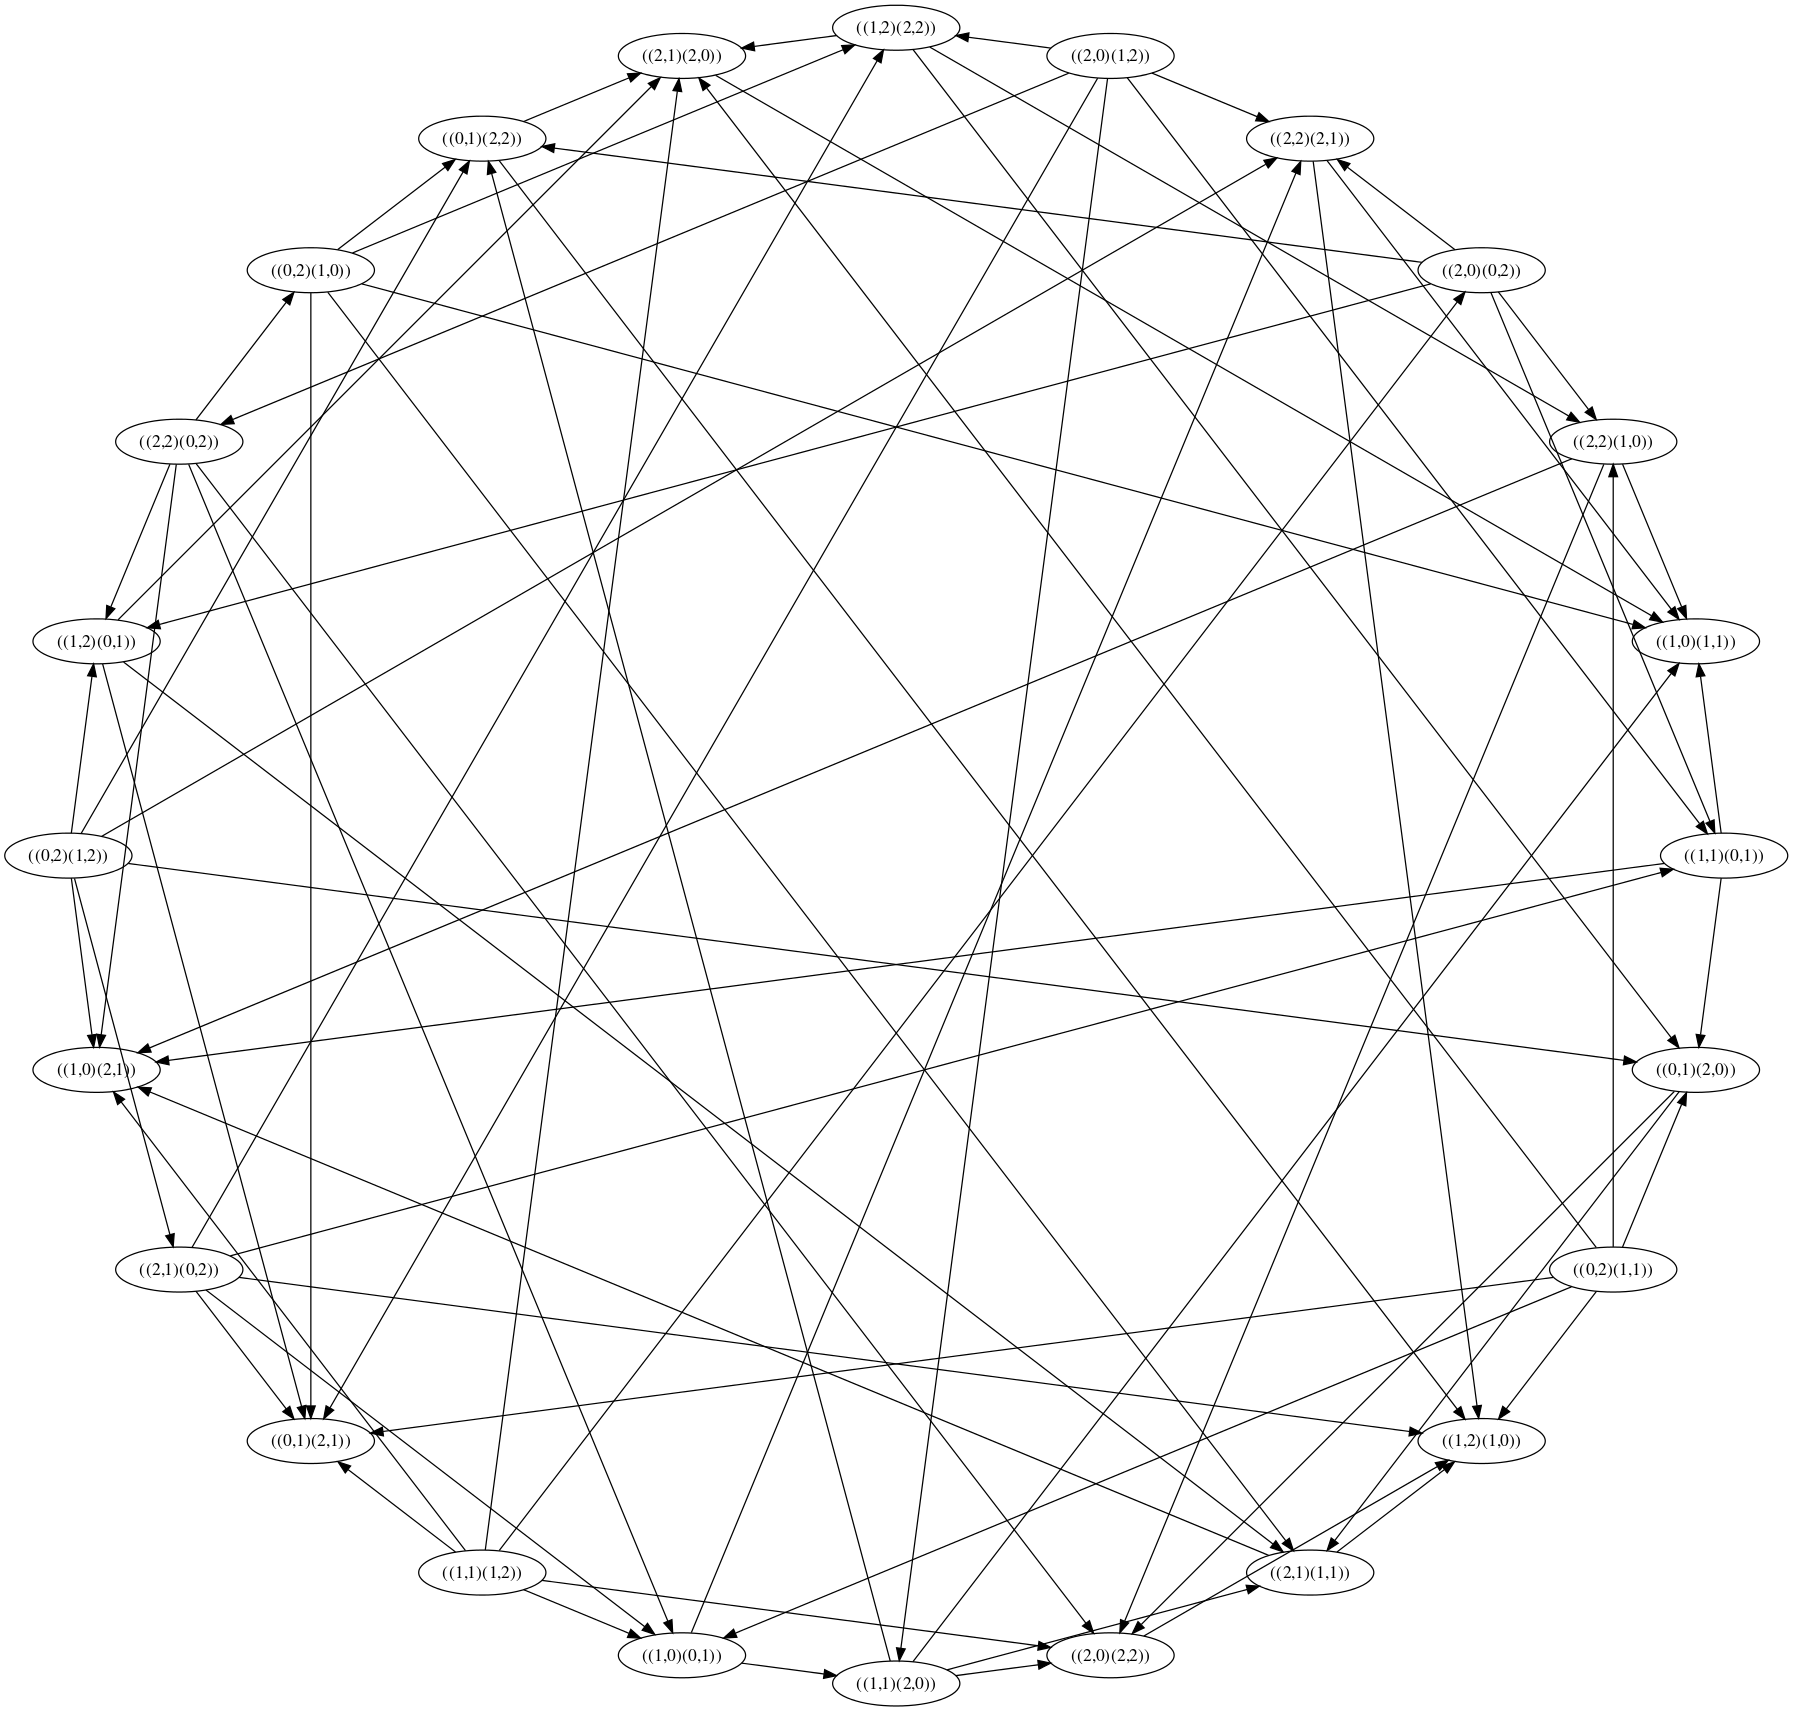
\includegraphics[scale=0.12]{example.png}
		\caption{One of the generated graphs from $SL(2,3)$ }
	\end{figure}
\end{frame}
%------------------------------------------------
\begin{frame}
	\frametitle{Further research}
	\begin{itemize}
		\item Finding smallest graph with given girth and degree is konwn as Degree/girth problem. With small changes to program we can systematically or randomly look for Cayley graphs and check its girth.
		\item Computations to find smallest graphs with $k=2$ in bigger Galois fields .
	\end{itemize}
\end{frame}
%------------------------------------------------
\begin{frame}
\Huge{\centerline{The End}}
\end{frame}
%----------------------------------------------------------------------------------------
\end{document} 

\begin{frame}
	\frametitle{Computer search of Cayley graphs}
	We know that Cayley graph is lift of one vertex with $|S|$ edges. We exploit that property by computation of diameter on smaller graph to determine it.
	\begin{theorem}[Diameter of Cayley graph]
		Cayley graph $(\Gamma, S)$ has diameter $k$ if and only if \\
		$ \forall x \in Cay(\Gamma, S) there \exists x_{1}, x_{2}, \dots ,x_{i} \in S$
	\end{theorem}
\end{frame}
